\documentclass{article}
% \linespread{1}

% if you need to pass options to natbib, use, e.g.:
% \PassOptionsToPackage{numbers, compress}{natbib}
% before loading nips_2017
%
% to avoid loading the natbib package, add option nonatbib:
% \usepackage[nonatbib]{nips_2017}

%\usepackage{main}

% to compile a camera-ready version, add the [final] option, e.g.:
\usepackage[final]{main}

\usepackage[utf8]{inputenc} % allow utf-8 input
\usepackage[T1]{fontenc}    % use 8-bit T1 fonts
\usepackage{hyperref}       % hyperlinks
\usepackage{url}            % simple URL typesetting
\usepackage{booktabs}       % professional-quality tables
\usepackage{amsfonts}       % blackboard math symbols
\usepackage{nicefrac}       % compact symbols for 1/2, etc.
\usepackage{microtype}      % microtypography
\usepackage{multicol}
\usepackage{graphicx}
\usepackage{amsmath}
\usepackage{bm}

\title{Visual Question Answering:\\Basic Algorithms Analysis and Comparison}
\graphicspath{{images/}}
\setcitestyle{square,sort,comma,numbers}

% The \author macro works with any number of authors. There are two
% commands used to separate the names and addresses of multiple
% authors: \And \AND.
%
% Using \And between authors leaves it to LaTeX to determine where to
% break the lines. Using \AND forces a line break at that point. So,
% if LaTeX puts 3 of 4 authors names on the first line, and the last
% on the second line, try using \AND instead of \And before the third
% author name.

\author{
  Daniel Rivera Ruiz\\
  Department of Computer Science\\
  New York University\\
  \href{mailto:drr342@nyu.edu}{\texttt{daniel.rivera@nyu.edu}}\\
}

\begin{document}
% \nipsfinalcopy is no longer used

\maketitle

\begin{abstract}
Visual Question Answering (VQA) is a challenging task that in recent years has gained a lot of attention both from the Computer Vision (CV) and Natural Language Processing (NLP) communities. Given an image and a natural language question, VQA requires visual reasoning and text inference knowledge in order to predict a correct answer to the question. This paper focuses on some of the algorithms proposed to solve this task in recent years, which usually rely on convolutional neural networks (CNN) to extract features from the input images and recurrent neural networks (RNN) to extract features from the input questions and map them to a common feature space. In addition to these modules, most methods incorporate an attention mechanism, which helps them to focus on specific regions of the input that are the most relevant to output the correct answer.
\end{abstract}

\section{Introduction}\label{intro}
For the task of VQA, the goal is to predict the most likely answer $\hat{a}$ for a given image $\bm{x}$ and question or phrase $\bm{q}$. This can be formulated as 
\begin{equation*}
    \hat{a} = \underset{a \in A}{\text{argmax}}\;p(a|\bm{x},\bm{q};\theta)
\end{equation*}
with model parameters $\theta$ and a set of answers $A$. The different methods presented throughout this paper propose several algorithms to solve this problem.\\
Within the frame of Artificial Intelligence (AI), VQA makes for a compelling "AI-complete" task because it requires multi-modal knowledge beyond a single sub-domain (Computer Vision, Natural Language Processing and Knowledge Representation and Reasoning) and because it has a well-defined quantitative evaluation metric, which will be explained in detail in section \ref{vqaSec}.\\
The interdisciplinary nature of the VQA problem along with the advent of deep learning techniques that allow for complex models to be computationally feasible and easily implemented, has contributed to the increasing popularity of the task among several communities within the computer science field, which has in turn has resulted in the publication of several papers on the subject in recent years.\\
The rest of this paper is organized as follows: in section \ref{vqaSec} we present the VQA dataset, which was introduced in 2015 and has ever since been the default dataset to develop and test VQA models. The baseline model published originally with the dataset is also explained in this section. Sections \ref{hiercoattSec} through \ref{dualnetSec} present seven models that have been developed ever since: Hierarchical Co-Attention, Stacked Attention Networks, Multimodal Residual Learning, Focused Dynamic Attention, Dynamic Memory Networks, Multimodal Compact Bilinear Pooling and the DualNet architecture. For each one of these models we present a brief explanation of the underlying algorithm and the experimental setup utilized by the original authors to achieve the results published. Section \ref{resSec} presents a summary of all the models, including a comparison of the algorithms and the results obtained. Section \ref{newSec} presents a new version of the VQA dataset, which was published in 2017 and modifies the original dataset, making it more balanced and less prone to bias due to language priors. Finally, sections \ref{futureSec} and \ref{conclusions} present guidelines for future work and the conclusions of the paper.

\section{VQA: Visual Question Answering}\label{vqaSec}
In this paper, Antol et al. propose the task of a free-form and open-ended VQA: given an image and a natural language question, the task is to provide an accurate natural language answer \citep{iccvAntol15}.\\
Before the advent of the VQA dataset, the efforts in the field where usually limited to a predefined closed set of possible answers, like 16 basic colors or a couple of hundred object categories. Also, the questions considered where usually generated from templates, which made them easier to respond without any real understanding of the associated image.
\subsection{The Dataset}
The VQA dataset contains 204,721 images from the MS COCO dataset as well as 50,000 abstract scenes constructed specifically with VQA in mind. Three questions were collected for each image or scene and each question was answered by ten subjects for a total of over 760,000 questions and 1 million answers. The real images are split following the same strategy as the original COCO dataset (including test-dev, test-std, test-challenge and test-reserve). For the abstract scenes they use a standard split with 20K/10K/20K for train/val/test, respectively.\\
The dataset is developed as follows:
\begin{enumerate}
    \item Questions are designed so that they require the image to be correctly answered, and not only using commonsense information.
    \item Human subjects are posed the following challenge: \emph{"We have built a smart robot. It understands a lot about images. It can recognize and name all the objects, it knows where the objects are, it can recognize the scene, people's expressions and poses, and properties of objects. Your task is to stump this smart robot!"}
    \item 10 answers for each question from unique workers are gathered, ensuring that the worker answering the question did not ask it.
\end{enumerate}
Some examples of the kind of images and questions that conform the dataset are depicted in figure \ref{questions}.

    \begin{figure}[ht]
    	\centering
            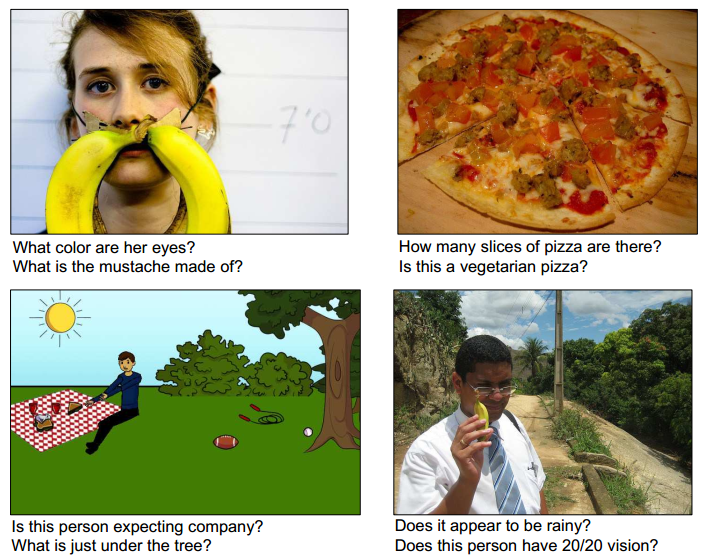
\includegraphics[width=0.75\linewidth]{questions.PNG}
    	\caption{Examples of the image-questions pairs available in the VQA dataset.}
    	\label{questions}
    \end{figure}
    
For testing, there are two modalities for answering the questions: open-answer and multiple-choice. For open-answer questions, the following accuracy metric is used: min$\left(\frac{\text{\# humans that provided the answer}}{3}, 1\right)$. This means that an answer is considered 100\% accurate if at least 3 workers provided that exact answer. For the multi-choice task, 18 candidate answer are generated for each question: 1 correct answer (the most common out of ten correct answers), 3 plausible answers (answers by three subjects without seeing the image), the 10 most popular answers (overall). After obtaining the union of these 3 categories, the remaining answers to complete 18 are drawn randomly from the correct answers bank for the whole dataset. The order of the answers is randomized. Figure \ref{q+ans} shows an example of an image with a couple of questions, along with correct and plausible answers.

    \begin{figure}[ht]
    	\centering
            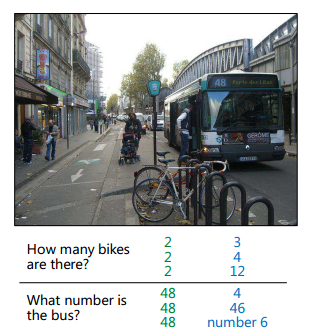
\includegraphics[width=0.5\linewidth]{q+ans.PNG}
    	\caption{Instance of an image-question of the VQA dataset, along with the correct answers for the question (green) and the plausible answers generated without looking at the image (blue).}
    	\label{q+ans}
    \end{figure}
 
\subsection{Dataset Analysis}
The clusters of question types according to the words that start the question are depicted in figure \ref{qdist}. The distribution of questions is quite similar for both real images and abstract scenes. Similarly, a distribution over type of answers is depicted in figure \ref{ansdist}. A number of questions such as "Is the...", "Does..." are typically answered using "yes" or "no", whereas questions like "What is..." or "What type..." have a much richer diversity of responses.\\
Most answers, however, consist of a single word, with the distribution of answers containing one, two or three words respectively being 89.32\%, 6.91\% and 2.74\% for real images. This is in contrast with the related problem of image captioning, where the expected result generically describes the entire image and hence tends to be longer.\\
On average, each question has 2.70 unique answers for real images and 2.39 for abstract scenes. Also, there is an inter-human agreement  of 83.30\% for real images and 87.49\% for abstract scenes, which increases significantly for "yes/no" questions (> 95\%) and decreases for "other" questions (< 76\%).

    \begin{figure}[ht]
    	\centering
            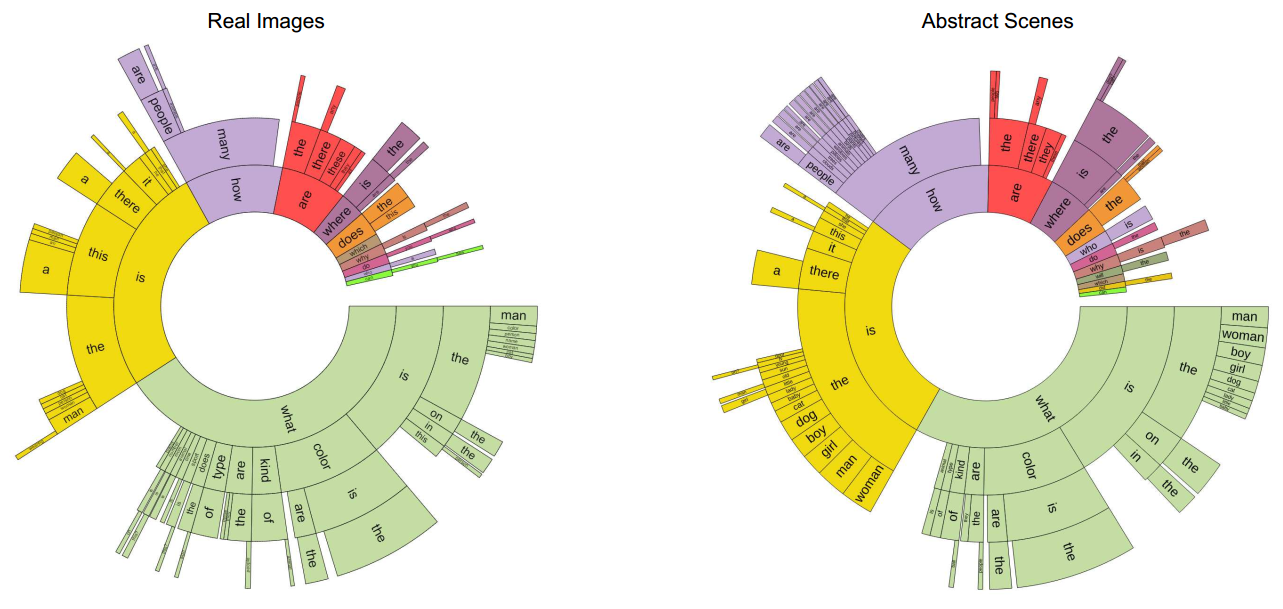
\includegraphics[width=1.0\linewidth]{qdist.PNG}
    	\caption{Distribution over the questions of the VQA dataset according to the first word of the question, both for real images and for abstract scenes.}
    	\label{qdist}
    \end{figure}
    \begin{figure}[ht]
    	\centering
            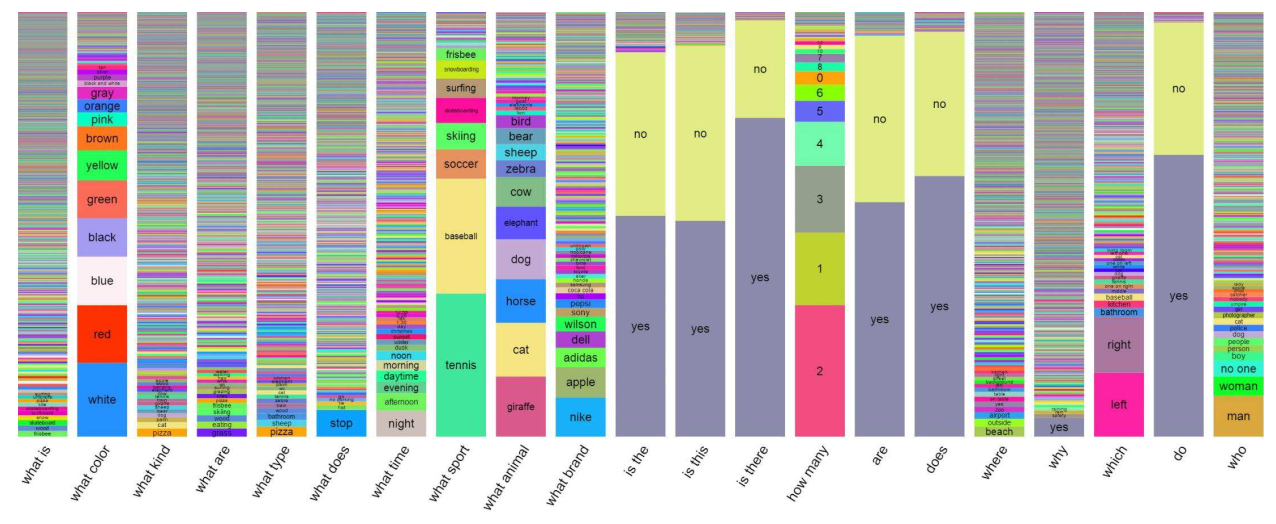
\includegraphics[width=1.0\linewidth]{ansdist.PNG}
    	\caption{Distribution over the answers of the VQA dataset for different kinds of questions.}
    	\label{ansdist}
    \end{figure}

\subsection{Baselines and methods}
Randomly choosing an answer from the top 1K answers of the VQA train/val dataset, the test-std accuracy is 0.12\%. Always selecting the most popular answer ("yes") yields a 29.72\% accuracy and picking the most popular answer per question type yields 36.18\%.
The model proposed is an LSTM that used one-hot encoding for the question words, and the last hidden layer of VGGNet as a 4096-dim feature vector for the images. A linear transformation is used to map the image features to 1024 dimensions and match the LSTM encoding of the question. The question and image encodings are fused via element-wise multiplication followed by a softmax layer to generate the answer. For the open-answer task, the model selects the answer with higher activation from all possible $K=1000$ answers, and for multiple-choice it picks the answer with the highest activation from the potential answers.\\
% A summary of the results can be found in table \ref{t1}. Additionally, a breakdown of accuracy by question type can be found in table \ref{t2}. From these tables it is evident that the proposed method falls short when compared to the results achieved by humans.

\section{Hierarchical Question-Image Co-Attention for VQA}\label{hiercoattSec}
In this paper, Lu et al. \citep{nipsLu16} propose that in addition to modeling "where to look" (visual attention), it is equally important to model "what words to listen to" (question attention), introducing a co-attention model for VQA which jointly reasons about these two factors.\\
Additionally, they develop a question hierarchy architecture that co-attends to the image and question at three levels: word, phrase and question. At the word level, words are embedded to a vector space through an embedding matrix. At the phrase level, 1-dimensional CNNs are used to capture the information contained in unigrams, bigrams and trigrams and the various responses are combined by pooling them into a single representation. At the question level, RNNs are used to encode the entire question. Figure \ref{coattModel} shows a graphical representation of the Hierarchical Question-Image Co-Attention model.

    \begin{figure}[ht]
    	\centering
            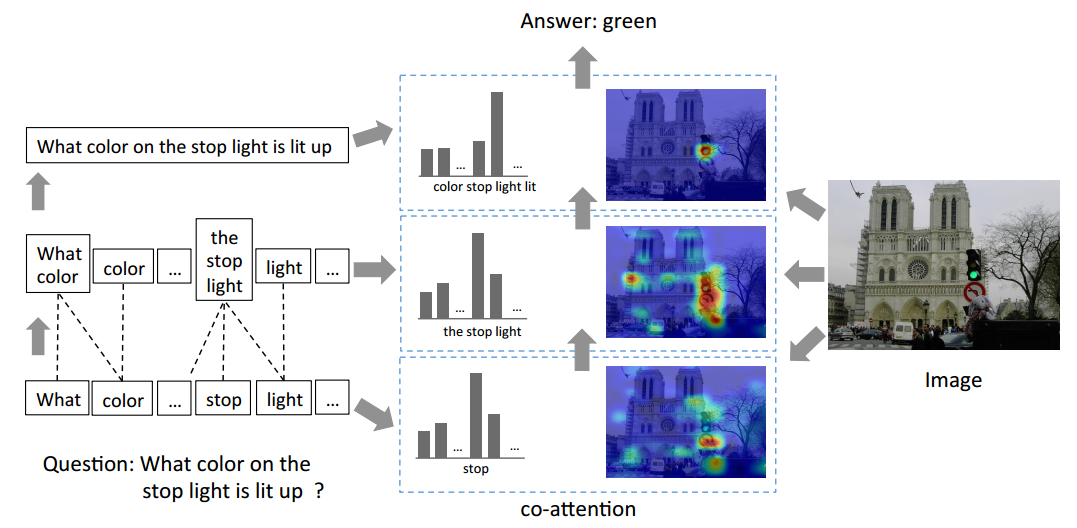
\includegraphics[width=0.75\linewidth]{coattModel.PNG}
    	\caption{Diagram for the Hierarchical Co-Attention Model.}
    	\label{coattModel}
    \end{figure}

\subsection{Hierarchy}
First, the words are embedded to a vector space to get $\bm{Q}^w=\{\bm{q}_1^w, \bm{q}_2^w, \ldots, \bm{q}_T^w\}$. For the phrase features, 1-D convolution is applied to the word vectors and max-pooling across different n-grams at each word adaptively selects the features at each time step:
\begin{align*}
    \hat{\bm{q}}_{s,t}^p &= \text{tanh}(\bm{W}_c^s\bm{q}_{t:t+s-1}^w), \quad s\in \{1, 2, 3\}\\
    \bm{q}_{s,t}^p &= \max(\hat{\bm{q}}_{1,t}^p, \hat{\bm{q}}_{2,t}^p, \hat{\bm{q}}_{3,t}^p)
\end{align*}
Finally, an LSTM encodes the sequence $\bm{q}_t^p$ to get the corresponding question-level feature $\bm{q}_t^s$ as the LSTM hidden vector at time $t$. The hierarchical representation of the question can be found in figure \ref{hierarchy+prediction} (a).

    \begin{figure}[ht]
    	\centering
            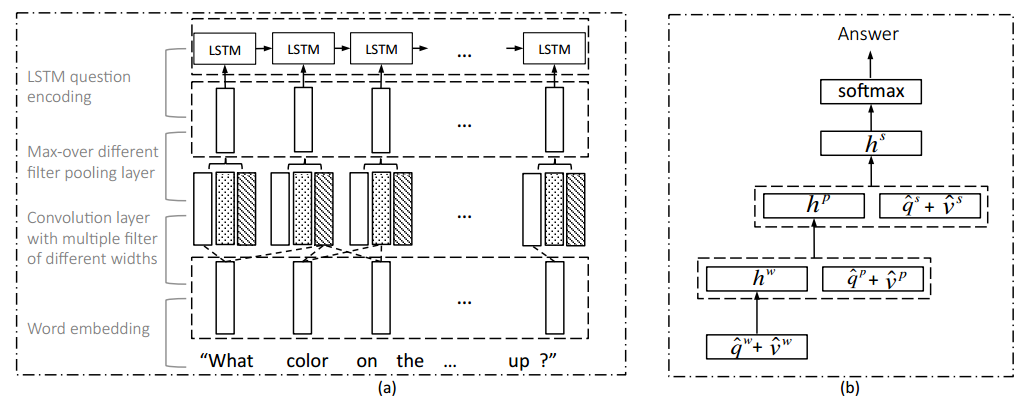
\includegraphics[width=1.0\linewidth]{hierarchy+prediction.PNG}
    	\caption{\textbf{(a)} Three-level hierarchy introduced by the HieCoAtt model at the question level, \textbf{(b)} Recursive multilayer perceptron used for prediction by the HieCoAtt model.}
    	\label{hierarchy+prediction}
    \end{figure}

\subsection{Parallel Co-Attention}
In this method, image and question attentions are generated simultaneously. Given an affinity matrix defined by
\begin{equation*}
    \bm{C} = \text{tanh}(\bm{Q}^T\bm{W}_b\bm{V})
\end{equation*}
that is used to transform question attention space to image attention space (vice versa for $\bm{C}^T$), the image and question attention maps are learned via the following:
\begin{align*}
    \bm{H}^v = \text{tanh}(\bm{W}_v\bm{V} + (\bm{W}_q\bm{Q})\bm{C}), &\quad \bm{H}^q = \text{tanh}(\bm{W}_q\bm{Q} + (\bm{W}_v\bm{V})\bm{C}^T)\\
    \bm{a}^v = \text{softmax}(w_{hv}^T\bm{H}^v), &\quad \bm{a}^q = \text{softmax}(w_{hq}^T\bm{H}^q)
\end{align*}
Where all the $w$ and $\bm{W}$ are weight parameters of the model and $\bm{a}^v$ and $\bm{a}^q$ are the attention probabilities. Based on these probabilities, the attention vectors are calculated as weighted sums:
\begin{equation*}
    \hat{\bm{v}} = \sum_{n=1}^Na_n^v\bm{v}_n, \quad \hat{\bm{q}} = \sum_{t=1}^Ta_t^q\bm{q}_t
\end{equation*}
Figure \ref{coattModels} (a) shows the Parallel Co-Attention Model.
\subsection{Alternating Co-Attention}
In this method, the image and question attentions are sequentially alternated, summarizing the question first, attending to the image using the question summary next, and finally attending to the question based on the attended image feature. Thus, thee attention operator is defined as follows
\begin{align*}
    \bm{H} &= \text{tanh}(\bm{W}_x\bm{X} + (\bm{W}_g\bm{g})\bm{1}^T)\\
    \bm{a}^x &= \text{softmax}(w_{hx}^T\bm{H})\\
    \hat{\bm{x}} &= \sum a_i^x\bm{x}_i
\end{align*}
where $\bm{x}$ can be either $\bm{q}$ or $\bm{v}$ depending on the step that is being performed. The attention guidance $\bm{g}$ is clearly equals to $\bm{v}$ when $\bm{x}$ is $\bm{q}$ and vice versa.
Figure \ref{coattModels} (b) shows the Alternation Co-Attention Model.

    \begin{figure}[ht]
    	\centering
            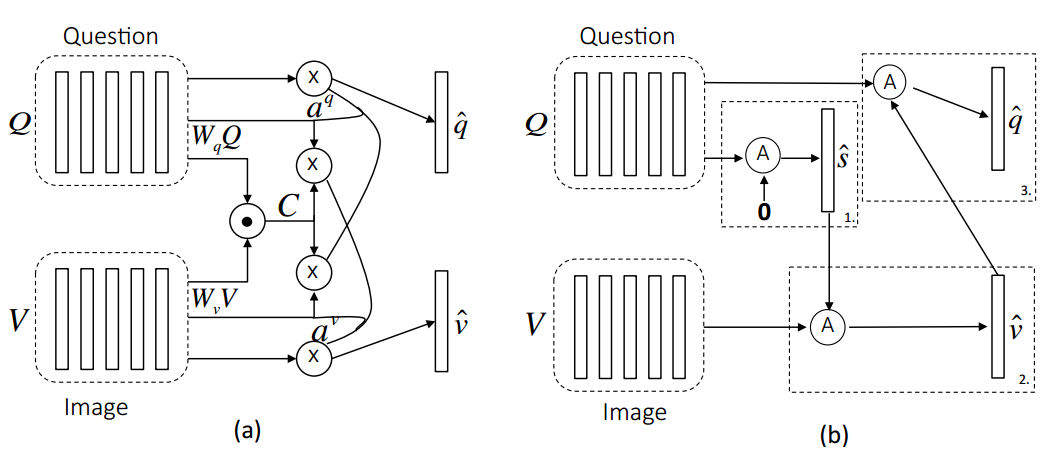
\includegraphics[width=0.75\linewidth]{coattModels.PNG}
    	\caption{\textbf{(a)} Parallel Co-Attention Model, \textbf{(b)} Alternating Co-Attention Model.}
    	\label{coattModels}
    \end{figure}

\subsection{Predicting answers}
A multilayer perceptron (MLP) is used to recursively encode the attention features:
\begin{align*}
    \bm{h}^w &= \text{tanh}(\bm{W}_w(\hat{\bm{q}}^w + \hat{\bm{v}}^w))\\
    \bm{h}^p &= \text{tanh}(\bm{W}_p[(\hat{\bm{q}}^p + \hat{\bm{v}}^p);\bm{h}^w])\\
    \bm{h}^s &= \text{tanh}(\bm{W}_s[(\hat{\bm{q}}^s + \hat{\bm{v}}^s);\bm{h}^p])\\
    p &= \text{softmax}(\bm{W}_h\bm{h}^s)
\end{align*}
where $[\cdot]$ is the concatenation operation and $p$ is the probability of the final answer. Figure \ref{hierarchy+prediction} (b) depicts this prediction model.\\
To setup the experiments, the top 1000 most frequent answers are used as the possible outputs just as in \citep{iccvAntol15}. The Rmsprop optimizer is used with learning rate 4e-4, momentum 0.99 and weight-decay 1e-8. The batch size is set to 300 and the model trained for 256 epochs with early stopping if the validation accuracy has not improved in the last 5 epochs. The size of $\bm{W}_s$ is set to 1024, while all other word embeddings and hidden layers are vectors of size 512. Dropout with probability 0.5 is applied on each layer, and the input images are rescaled to $4448 \times 448$ before taking the activation from the last pooling layer of VGGNet or ResNet as its feature. Examples of the attention maps generated during the experiments are available in figure \ref{coattMaps}.

    \begin{figure}[ht]
    	\centering
            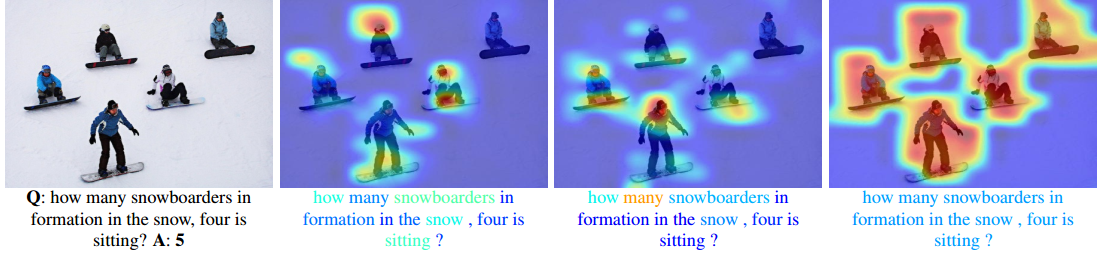
\includegraphics[width=1.0\linewidth]{coattMaps.PNG}
    	\caption{From left to right: input image, attention maps at the word level, attention maps at the phrase level, attention maps at the question (sentence) level.}
    	\label{coattMaps}
    \end{figure}
    
\section{Stacked Attention Networks for Image Question Answering}
In this paper, Yang et al. \citep{corrYang15} propose a model called Stacked Attention Networks (SAN) that allows multi-step reasoning for the VQA problem. The SAN model can be viewed as an extension of the attention mechanism that has been successfully applied to image captioning and machine translation, and consists of three major components: image model, question model and stacked attention model, which locates the image regions that are relevant to the question for answer predictions.\\
The SAN first uses the question vector to query the image in the first visual attention layer. The results are combined with the question vector to form a refined query that goes to the second visual attention layer, which in turn gives a sharper attention distribution focusing on the regions that are more relevant to the answer. The features of the highest attention layer and the last query vector are combined to predict the answer.
\subsection{The Model}
The image model uses a CNN, specifically VGGNet, to extract the feature map $f_I$ from a raw image $I$. The features $f_I$ are taken from the last pooling layer of size $512 \times 14 \times 14$, which retains spatial information of the original images, which are rescaled to be $448 \times 448$. Finally, a single layer perceptron is used to transform each feature vector to a new vector that has the same dimension as the question vector: $v_I=\text{tanh}(W_If_I+b_I)$.\\
Unlike most approaches, SAN also uses a CNN instead of an LSTM to extract the features from the question. Given the word embeddings $x_t = W_eq_t$ for all words $q_t$, the question vector is formed by concatenation $x_{1:T} = [x_1,x_2,\ldots,x_T]$ and three convolution filters for unigrams, bigrams and trigrams are used. The $t$-th convolution output for window size $c$ is given by $h_{c,t} = \text{tanh}(W_cx_{t:t+c-1}+b_c)$. Applying max-pooling over the feature maps for convolution size $c$ and concatenating for sizes $c = \{1, 2, 3\}$ yields
\begin{align*}
    \Tilde{h}_c &= \max[h_{c,1}, h_{c,2},\ldots,h_{c,T-c+1}]\\
    h &= [\Tilde{h}_1, \Tilde{h}_2, \Tilde{h}_3]
\end{align*}
and thus $v_Q = h$ is the CNN based question vector. This CNN architecture is depicted in figure \ref{sanCNN}.\\

    \begin{figure}[ht]
    	\centering
            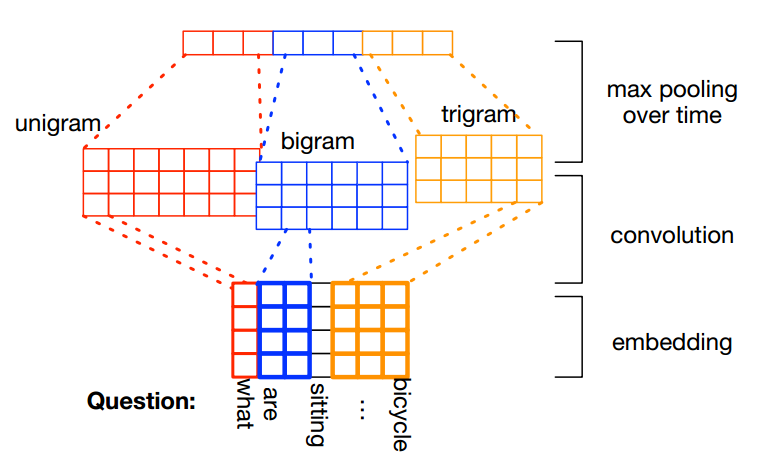
\includegraphics[width=0.75\linewidth]{sanCNN.PNG}
    	\caption{CNN model used by SAN for question feature extraction.}
    	\label{sanCNN}
    \end{figure}

For the stacked attention model, a single layer neural network followed by a softmax function is used to generate the attention distribution over the image regions. After each iteration, the attention probabilities are used to update the image and question representations thus extracting more fine-grained visual information. The model at the $k$-th iteration is expressed as follows
\begin{align*}
    h_A^k &= \text{tanh}(W_{I,A}^kv_I \oplus (W_{Q,A}^ku^{k-1} + b_A^k))\\
    p_I^k &= softmax(W_p^kh_A^k + b_p^k)\\
    \Tilde{v}_I^k &= \sum p_i^kv_i\\
    u^k &= \Tilde{v}_I^k + u^{k-1}
\end{align*}
where $u^0 = v_Q$, $p_I^k \in \mathbb{R}^m$ is the vector which corresponds to the attention probability for each image region at step $k$, and $\oplus$ denotes addition of a matrix and a vector (adding each column of the matrix by the vector). After $K$ iterations, the final $u^K$ is used to infer the answer:
\begin{equation*}
    p_{ans} = \text{softmax}(W_uu^K + b_u)
\end{equation*}
Figure \ref{sanArch} shows a graphical representation of the whole SAN model.

    \begin{figure}[ht]
    	\centering
            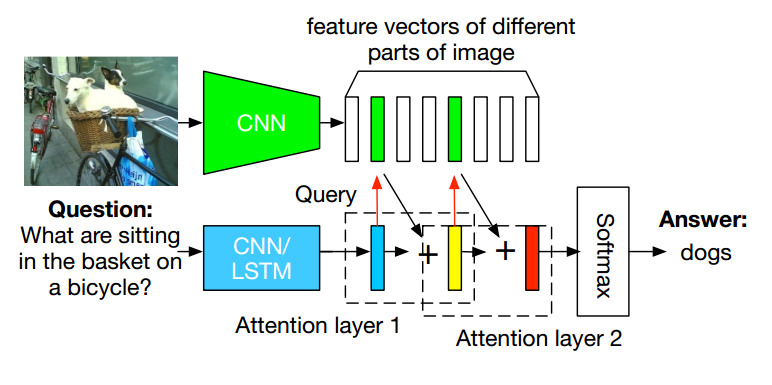
\includegraphics[width=0.75\linewidth]{sanArch.PNG}
    	\caption{Architecture of the SAN model.}
    	\label{sanArch}
    \end{figure}

\subsection{Experiments and Results}
The image features are taken from the last pooling layer of VGGNet, with dimensions $512 \times 14 \times 14$. The CNN question model uses convolution filter size 256, 512, 512 for unigram, bigram and trigram respectively, for an overall question vector size of 1280. During evaluation, only one and two attention layers are used (using three or more layers did not improve performance any further). All models were trained using SGD with momentum 0.9. The batch size was fixed to be 100 and the best learning rate was picked using grid search. Gradient clipping and dropout regularization are also used. Examples of the attention maps generated during training of the SAN model are depicted in figure \ref{sanMaps}.

    \begin{figure}[ht]
    	\centering
            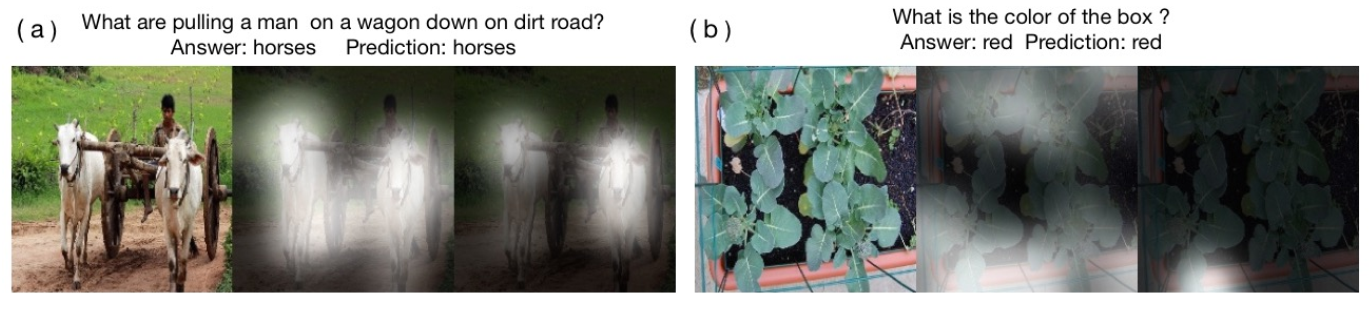
\includegraphics[width=1.0\linewidth]{sanMaps.PNG}
    	\caption{Two examples of the attention maps generated with SAN: the middle map corresponds to the first level of attention, the map to the right corresponds to the second level.}
    	\label{sanMaps}
    \end{figure}

\section{Multimodal Residual Learning for VQA}
In this paper, Kim et al. \citep{DBLP:corrKim16} introduce the idea of applying deep residual learning to the problem of VQA. The basic idea behind residual learning is that a block of deep neural networks forming a non-linear mapping $F(x)$ may paradoxically fail to fit an identity mapping. To resolve this, a shortcut connection to the input is added to $F$: $\bm{y} = F(\bm{x}) + \bm{x}$. Building on top of this and on the Stacked Attention Networks (SAN) model, an addition of the combined visual feature vector and the previous question vector is transferred as a new input question vector to the next learning block:
\begin{equation*}
    \bm{q}^k = F(\bm{q}^{k-1}, \bm{V}) + \bm{q}^{k-1}
\end{equation*}
where $\bm{q}^l$ is a question vector for the $l$-th learning block, $\bm{V}$ is a visual feature matrix and $F(\bm{q},\bm{V})$ has the form of the attention networks from the SAN model.\\
This approach emphasizes the importance of identity (or linear) shortcuts to have the non-linear mappings efficiently learn only the residuals. The overall flow of information of the Multimodal Residual Network (MRN) is depicted in figure \ref{mrnInference}.

    \begin{figure}[ht]
    	\centering
            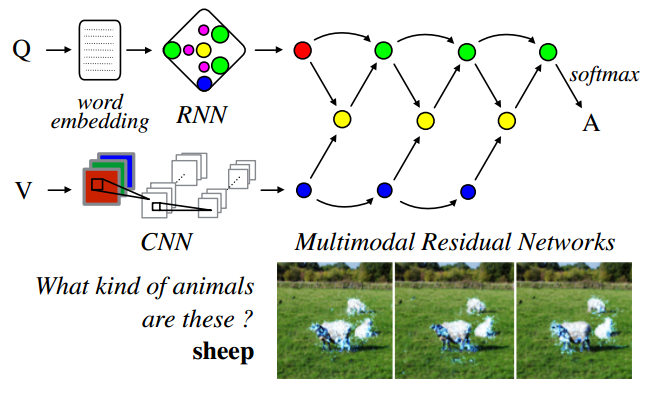
\includegraphics[width=0.5\linewidth]{mrnInference.PNG}
    	\caption{Dataflow at inference time for the Multimodal Residual Network.}
    	\label{mrnInference}
    \end{figure}

\subsection{The Model}
MRN consists of multiple learning blocks, which are stacked for deep residual learning. The optimal mapping at the first level of the network is given by
\begin{equation*}
    H_1(\bm{q},\bm{v}) = W_{\bm{q'}}^{(1)}\bm{q} + F^{(1)}(\bm{q},\bm{v})
\end{equation*}
where $W_{\bm{q'}}^{(1)}\bm{q}$ is the first linear approximation term ($W_{\bm{q'}}$ is used as a transformation for dimensionality match) and the joint residual function $F$ is defined as
\begin{equation*}
    F^{(k)}(\bm{q},\bm{v}) = \text{tanh}(W_{\bm{q}}^{(k)}\bm{q}\odot\text{tanh}(W_2^{(k)}\text{tanh}(W_1^{(k)}\bm{v}))
\end{equation*}
For a deeper residual learning $\bm{q}$ is replaced with $H_1(\bm{q},\bm{v})$ and the two equations can be rewritten as follows:
\begin{equation*}
    H_L(\bm{q},\bm{v}) = W_{\bm{q'}}\bm{q} + \sum_{l=1}^LW_{F^{(l)}}F^{(l)}(H_{l-1},\bm{v})
\end{equation*}
where $L$ is the number of learning blocks, $H_0 = \bm{q}, W_{\bm{q'}}=\prod_{l=1}^LW_{\bm{q'}}^{(l)}$, and $W_{F^{(l)}} = \prod_{m=l+1}^LW_{\bm{q'}}^{(m)}$. The cascading nature of the last equation is depicted graphically in figure \ref{mrnModel}, where the shortcuts for the linear and identity mappings are clearly shown.

    \begin{figure}[ht]
    	\centering
            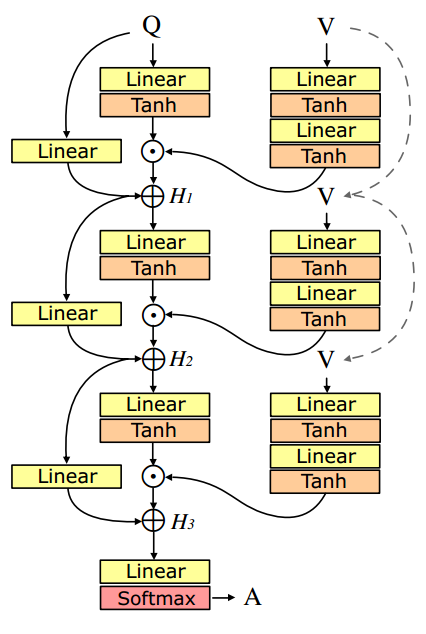
\includegraphics[width=0.35\linewidth]{mrnModel.PNG}
    	\caption{Architecture of the Multimodal Residual Network.}
    	\label{mrnModel}
    \end{figure}

\subsection{Experiments and Results}
To build the model, they use the Torch framework and the \emph{rnn} package along with \emph{TrimZero} to eliminate zero computations at every time-step in mini-batch learning, which reduces the training time in approximately 37.5\%.\\
Questions are tokenized using Python NLP Toolkit (nltk) and transformed to a vector $\bm{q} \in \mathbb{R}^{2,400}$ using the last output vector of a GRU with orthogonal initialization for all recurrent matrices and a uniform distribution in $[-0.1,0.1]$ for non-recurrent weights. The visual vector $\bm{v}$ is the output of the first fully-connected layer of VGG-19 network (dimension 4,096) or alternatively using ResNet-152 with dimension 2,048. The error is back-propagated to the input question for fine-tuning but not for the visual part due to the heavy computational cost.\\
The common embedding size of the joint representation is 1,200 and the learnable parameters (except for the pretrained models already described) are initialized using a uniform distribution in $[-0.08,0.08]$. The batch size is 200, the number of iterations is fixed to 250k, RMSProp is used for optimization and dropout for regularization.\\
The overall accuracies as the number of learning block increases are 58.85\% for $L=1$, 59.44\% for $L=2$, \textbf{60.53\%} for $L=3$ and 60.42\% for $L=4$. Even though the ResNet features have half the dimensions of the VGG-19 features, better performance is achieved with the former. 
\subsection{Qualitative Analysis and Implicit Attention}
In the expression for $F$, the left term $W_{\bm{q}}\bm{q}$ can be seen as a masking (attention) vector to select a part of visual information. Therefore, the difference between the right term of $F$ and $F$ itself indicates an attention effect caused by the masking vector, which gives the element-wise multiplication an interpretation of information masking. In this sense, the MRN model includes an implicit attention mechanism that has much higher resolution than most of the other methods that depend only on a few attention parameters. Examples of the high-resolution attention maps obtained with MRN are depicted in figure \ref{mrnMaps}.

    \begin{figure}[ht]
    	\centering
            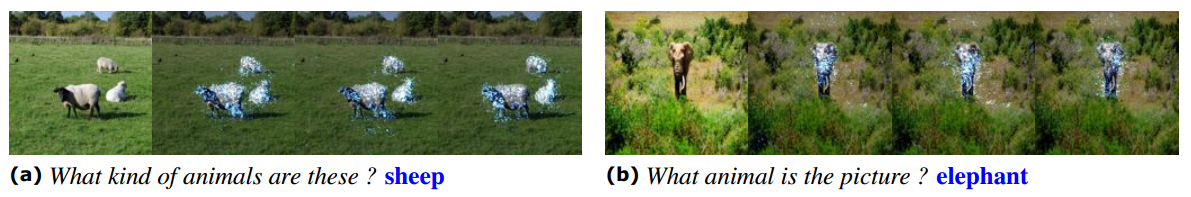
\includegraphics[width=1.0\linewidth]{mrnMaps.PNG}
    	\caption{Input gradients of the attention effect for each learning block of the MRN model, along with the corresponding input images (left).}
    	\label{mrnMaps}
    \end{figure}

\section{A Focused Dynamic Attention Model for VQA}
In this paper, Ilievski et al. \citep{corrIlievski16} introduce the Focused Dynamic Attention (FDA) model, which employs off-the-shelf object detection to identify important regions and fuse their information along with global features via an LSTM unit. Such question-driven representations are then combined with the question representation and fed into a reasoning unit to generate the final answer.\\
The logic behind this idea is that oftentimes VQA methods only extract global features from the image, which fails in capturing fine-grained information such as spatial configuration of multiple objects or informative background. Alternatively, using features from all the regions in the image could result in too much noise or overwhelming information irrelevant to the question.\\
The FDA model lies right in between these two approaches, being able to automatically identify and focus on image regions that are relevant for the question at hand. For instance, to answer the question "How many apples are in the basket?", FDA would first localize the regions corresponding to the key words "apples" and "basket" and extract description features of these regions of interest.
\subsection{The Model}
FDA uses an LSTM network to encode the question in a vector representation and a pre-trained ResNet model to extract image feature vectors. It uses the weights of the layer immediately before the final SoftMax layer and regard them as visual features. The visual features for the whole image and for the specific focus regions are combined in a joint representation via another LSTM.\\
The attention mechanism is based on similarity between the question words and the objects present in the image: If the word2vec embedding of an object’s label scores 0.5 or greater, the feature vectors of the bounding box containing the object are extracted using the pre-trained ResNet model. Following the question word order, the feature vectors are fed to the LSTM network followed by the feature vector of the global image. The resulting LSTM state is used as the visual representation.\\
Finally, the multimodal fusion is performed by applying \emph{tanh} on the question representation and \emph{ReLU} on the image representation. The two are brought together by element-wise multiplication and the resulting vector is fed to a fully-connected neural network. Finally, a softmax layer classifies the multimodal representation into one of the possible answers. A diagram of the FDA model is depicted in figure \ref{fdaModel}.

    \begin{figure}[ht]
    	\centering
            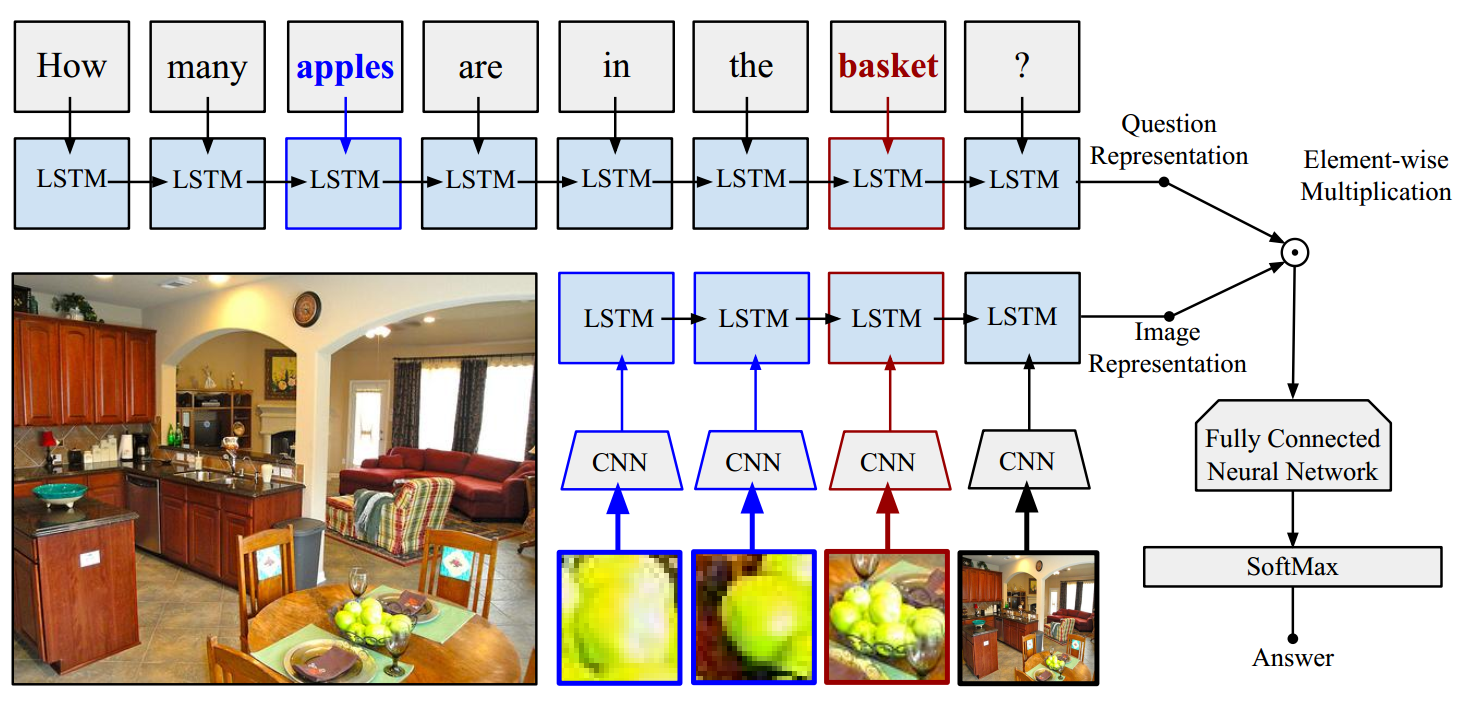
\includegraphics[width=0.75\linewidth]{fdaModel.PNG}
    	\caption{Focus Dynamic Attention (FDA) model diagram.}
    	\label{fdaModel}
    \end{figure}

Unlike the SAN model, where the attention focuses on more spread regions which may include cluttered and noisy background, this model benefits from the attention being focused on specific regions that are known to be relevant to the question. An example of the object-specific attention achieved with the FDA model is depicted in figure \ref{fdaExample}.

    \begin{figure}[ht]
    	\centering
            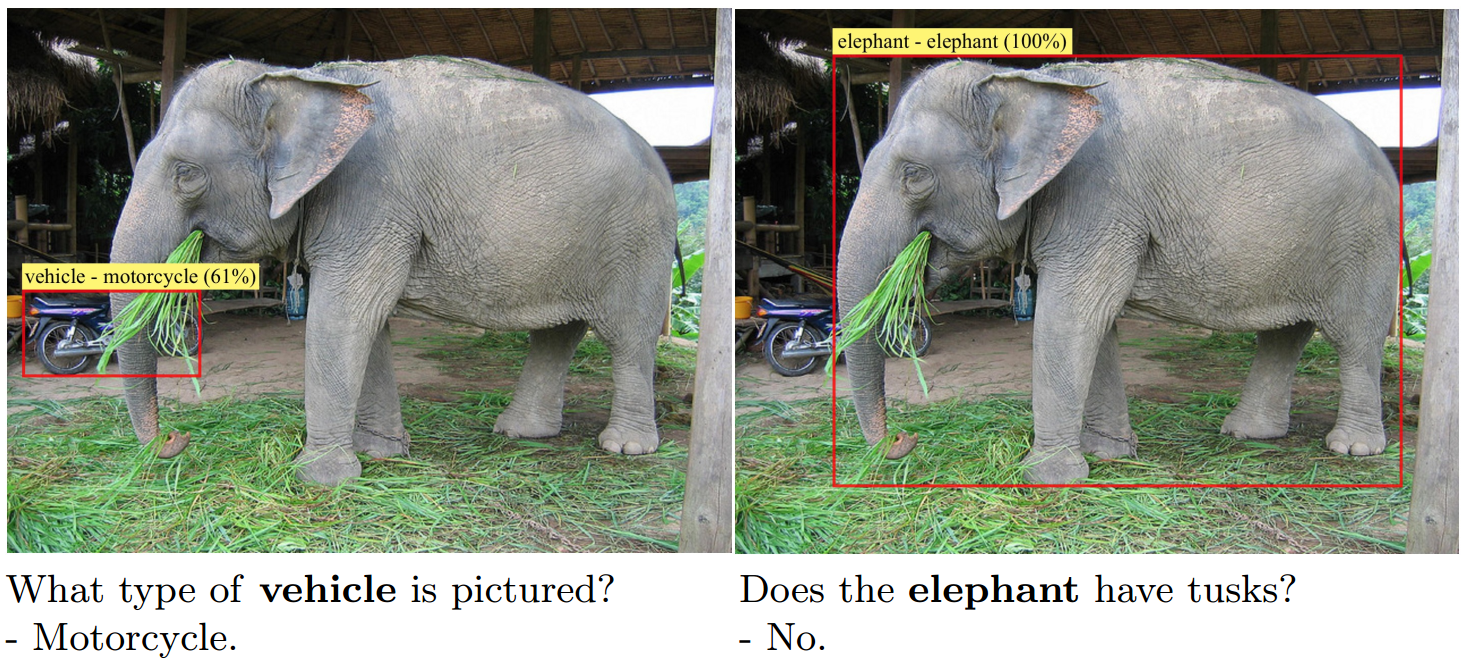
\includegraphics[width=0.75\linewidth]{fdaExample.PNG}
    	\caption{For the same image, the FDA model focuses  on different objects (depicted by the bounding box) depending on the question.}
    	\label{fdaExample}
    \end{figure}

\subsection{Experiments and Results}
The question words are transformed into vector form by multiplying the one-hot vector representation with a word embedding matrix. The resulting vocabulary size is 12,602 and the word embeddings are 300 dimensional. For the images, the 2,048-dimensional weight vector of the layer before the last fully-connected layer of ResNet is used. The LSTM networks used to bring the two representations together have a standard architecture with a 512-dimensional state vector.

\section{Dynamic Memory Networks for Visual and Textual QA}
In this paper, Xiong et al. \citep{corrXiong16} introduce the concept of a dynamic memory network (DMN) in the context of visual and textual QA. The DMN is a general architecture for question answering composed of  modules that allow different aspects such as input representations or memory components to be analyzed and improved independently.\\
In the original context of textual QA, the DMN consists of four modules (a graphical representation of a DMN is depicted in figure \ref{dmnArch}:
\begin{enumerate}
    \item Input module. processes the input data (text) about which a question is being asked into a set of ordered vectors known as facts. This module is implemented as a gated recurrent unit (GRU) over the input words.
    \item Question module. computes a vector representation $q$ of the question as the final hidden state of a GRU over the words in the question.
    \item Episodic memory module. it consists of the attention mechanism and the memory update mechanism, and it aims to retrieve information required to answer $q$ from the input facts. The attention mechanism is responsible for creating a context vector $c^t$ with a summary of relevant information, while the memory update generates the episodic memory $m^t$ that contains information from the context vector and previous episodic memory values.
    \item Answer module. it receives both $q$ and $m^T$ to generate the predicted answer, i.e. a linear layer with a softmax activation.
\end{enumerate}

    \begin{figure}[ht]
    	\centering
            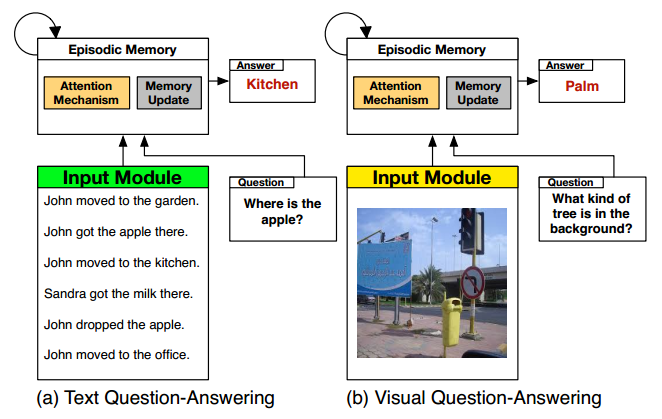
\includegraphics[width=0.75\linewidth]{dmnArch.PNG}
    	\caption{Architecture of the DMN model for \textbf{(a)} text QA and \textbf{(b)} visual QA.}
    	\label{dmnArch}
    \end{figure}

To apply these concepts to the problem of VQA, a couple modifications are implemented. First, the single GRU in the input module is replaced by a bi-directional GRU that will allow the facts to include context from regions that come before and after them. Also, this mechanism will allow for information to propagate among neighboring image regions, capturing spatial information. The resulting bidirectional facts $\overset{\longleftrightarrow}{f_i}$ are defined as follows:
\begin{align*}
    \overset{\longrightarrow}{f_i} &= GRU_{fwd}(f_i, \overset{\longrightarrow}{f_{i-1}})\\
    \overset{\longleftarrow}{f_i} &= GRU_{bwd}(f_i, \overset{\longleftarrow}{f_{i+1}})\\
    \overset{\longleftrightarrow}{f_i} &= \overset{\longleftarrow}{f_i} + \overset{\longrightarrow}{f_i}
\end{align*}
This module is built on top of the visual feature embeddings extracted from each region of the input image by using a VGG-19 CNN. As it is standard, the images are resized to $448 \times 448$ and the output from the last pooling layer ($d = 512 \times 14 \times 14$) is taken as the features. These features pass through a linear layer with \emph{tanh} activation to project them into the textual feature space used by the question vector $q$. Figure \ref{dmnInput} shows the modified input module for the VQA task.

    \begin{figure}[ht]
    	\centering
            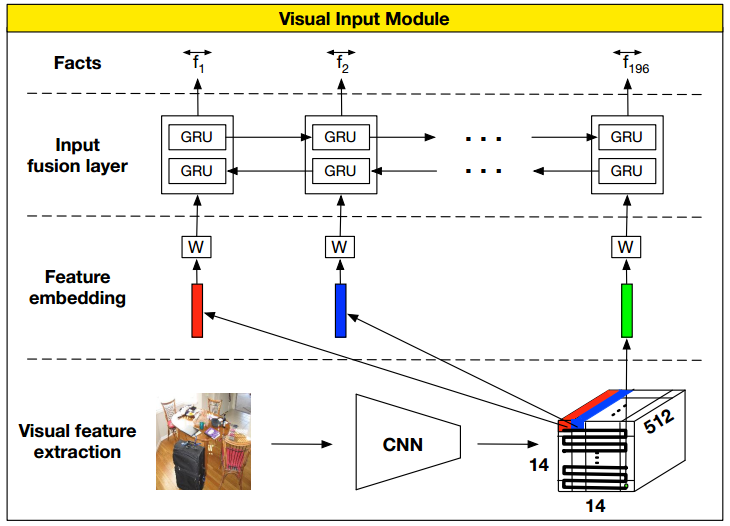
\includegraphics[width=0.75\linewidth]{dmnInput.PNG}
    	\caption{Modified input module of the DMN architecture for the VQA task.}
    	\label{dmnInput}
    \end{figure}

The episodic memory module is designed in such a way that the attention gates $g_i^t$ allow the interaction between facts, the question and the episode memory state:
\begin{align*}
    z_i^t &= [\overset{\longleftrightarrow}{f_i} \odot q; \overset{\longleftrightarrow}{f_i} \odot m^{t-1}; |\overset{\longleftrightarrow}{f_i} - q|; |\overset{\longleftrightarrow}{f_i} - m^{t-1}|]\\
    Z_i^t &= W^{(2)}\text{tanh}\left(W^{(1)}z_i^t+b^{(1)}\right) + b^{(2)}\\
    g_i^t &= \text{softmax}(Z_i^t)\\
\end{align*}
where $m^{t-1}$ is the previous episode memory, $\odot$ is element-wise multiplication, $|\cdot|$ is element-wise absolute value, and $[;]$ is concatenation.\\
These attention gates are used to replace the update gate $u_i$ in the GRU original model, which generates an attention-based architecture that is sensitive to both the position and ordering of the input facts. This attention based GRU will use $g_i^t$ to update its internal state as depicted in figure \ref{dmnGRU}. To produce the contextual vector $c^t$ used for updating the episodic memory state $m^t$, the final hidden state of the attention based GRU is used in the following expression:
\begin{equation*}
    m^t = ReLU(W^t[m^{t-1};c^t;q] + b)
\end{equation*}
The final output of the memory network is passed to the answer module as in the original DMN (linear layer with softmax activation). The episodic memory of the DMN architecture is depicted in figure \ref{dmnMemory}.

    \begin{figure}[ht]
    	\centering
            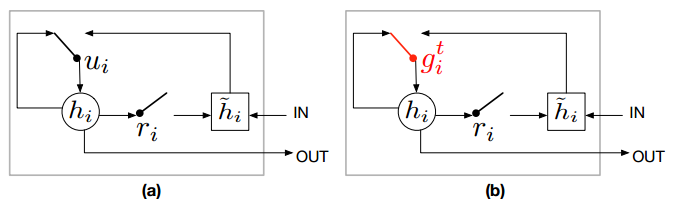
\includegraphics[width=0.75\linewidth]{dmnGRU.PNG}
    	\caption{Modified GRU network to incorporate attention gates $g_i^t$.}
    	\label{dmnGRU}
    \end{figure}
    \begin{figure}[ht]
    	\centering
            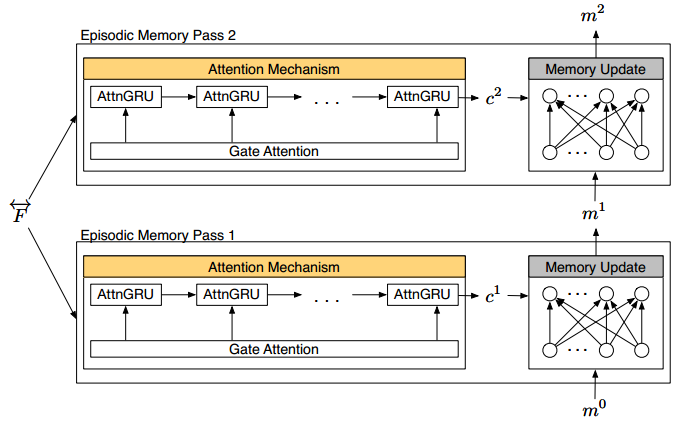
\includegraphics[width=0.75\linewidth]{dmnMemory.PNG}
    	\caption{Episodic memory module of the DMN model for VQA, including the attention GRU mechanism.}
    	\label{dmnMemory}
    \end{figure}

\subsection{Experiments and Results}
The resulting model, named DMN+, is an untied model that uses a unique set of weights for each pass. The Adam optimizer is implemented with learning rate of 0.003, batch size of 100 and training for 256 epochs with early stopping if the validation loss has not improved in the last 10 epochs. Weight initialization is drawn from a random uniform distribution with range $[-0.8,0.8]$. Both the word embeddings and hidden layers were vectors of size 512. Dropout with probability 0.5 was applied to the initial image output from the VGG CNN as well as the input to the answer module.

\section{Multimodal Compact Bilinear Pooling for VQA}
In this paper, Fukui et al. \citep{corrFukui16} introduce a new approach to multimodal pooling, which thus far had been modeled as an element-wise product or sum, as well as concatenation of visual and textual representations. While an outer product of these vectors can be much more expressive, it is also unfeasible due to its high dimensionality. As an alternative, Multimodal Compact Bilinear pooling (MCB) is introduced to efficiently and expressively combine multimodal features.\\
Recurrent neural networks (usually in the form of LSTMs) are often used to represent sentences or phrases, while CNNs have shown to work best for representing images. For tasks such as VQA, the representations of both modalities must somehow be integrated. Bilinear pooling computes the outer product between two vectors, which allows a multiplicative interaction between all elements. However, given the high dimensionality ($n^2$) it introduces, it has not been widely used.\\
Compact Bilinear pooling is an approximation that randomly projects the image and text representations to a higher dimension space and then convolves both vectors efficiently by using element-wise product in Fast Fourier Transform (FFT) space.
\subsection{MCB}
The main reasoning underlying the MCB method is to take an image embedding $x = \Xi(\bm{x})$ and a question embedding $q=\Omega(\bm{q})$ and encode their relationship via an MCB: $\Phi(x,q)$.\\
If $\phi$ were to be calculated directly as the outer product, i.e. $W[x \otimes q]$, where $\otimes$ denotes the outer product and $[\cdot]$ denotes linearizing the matrix into a vector, the weight matrix W would have 12.5 billion parameters for inputs of dimension 2048 and output of dimension 3000. Thus, a method to project the outer product to a lower dimensional space and to avoid computing it directly is required.\\
The Count Sketch projection function $\Psi$ helps with the dimensionality reduction: it projects a vector $v \in \mathbb{R}^n$ to $y \in \mathbb{R}^d$, where $n < d < n^2$. To achieve this, two auxiliary vectors $s$ and $h$ (initialized randomly from a uniform distribution) are used according to lines 1-9 and 12-16 in Algorithm 1.\\
Once the outer product is projected to a lower dimensional space, the algorithm benefits from the fact that the outer product of two vectors can be expressed as convolution of both count sketches:
\begin{equation*}
    \Psi(x \otimes q, h, s) = \Psi(x, h, s) * \Psi(q, h, s)
\end{equation*}
Furthermore, the convolution theorem states that convolution in the time domain is equivalent to element-wise product in the frequency domain. Therefore, the convolution $x'*q'$ can be rewritten as $\text{FFT}^{-1}(\text{FFT}(x')\odot\text{FFT}(q'))$. These ideas are summarized graphically in figure \ref{mcb} and formalized in Algorithm 1.

    \begin{figure}[ht]
    	\centering
            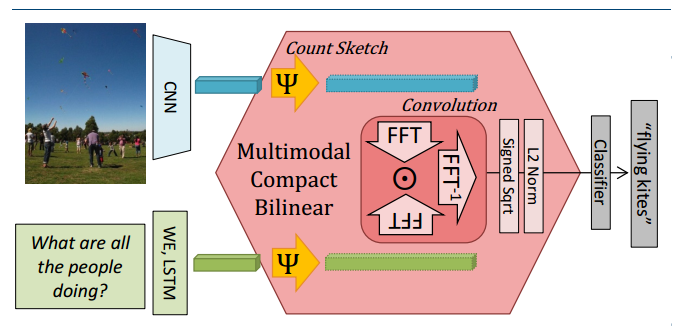
\includegraphics[width=0.5\linewidth]{mcb.PNG}
    	\caption{Multimodal Compact Bilinear Pooling for visual question answering.}
    	\label{mcb}
    \end{figure}
    \begin{figure}[ht]
    	\centering
            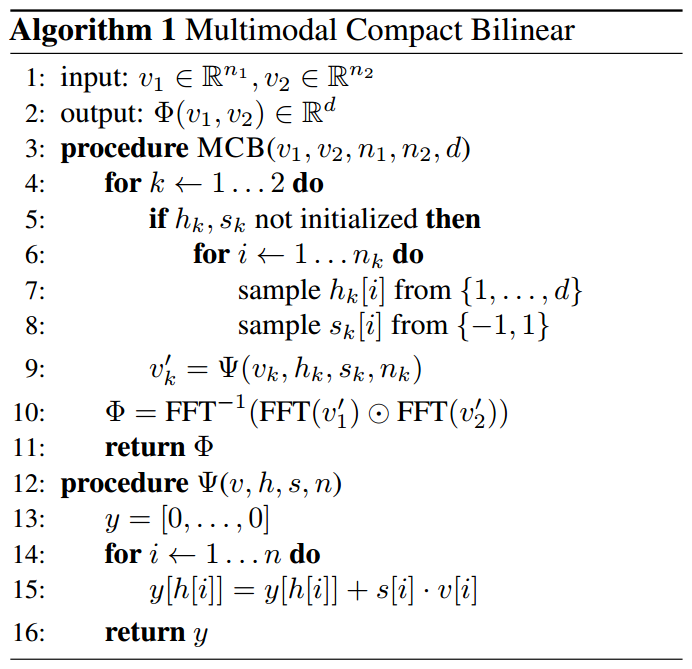
\includegraphics[width=0.5\linewidth]{mcbAlgo.PNG}
    	\label{mcbAlgo}
    \end{figure}

\subsection{Architecture}
The model extracts representations for the image and the question, pools the vectors using MCB and arrives at the answer by treating the problem as a multi-class classification problem with 3,000 possible classes.\\
The image features are extracted from a 152-layer ResNet pretrained on ImageNet data. Images are resized to $448 \times 448$ and the output of the layer before the 1000-way classifier is used. Finally, $L_2$ normalization is performed on the 2048-D vector.\\
Input questions are tokenized into words and the words are one-hot encoded and passed through a learned embedding layer followed by a tanh to introduce nonlinearity. The embedding layer is followed by a 2-layer LSTM with 1024 in each layer. The outputs of each LSTM layer are concatenated to form a 2048-D vector. The two vectors are then passed through MCB followed by an element-wise signed square-root, $L_2$ normalization, a fully connected layer and a softmax to generate the final prediction.\\
Additionally, two elements can be incorporated to the model:
\begin{itemize}
    \item Attention. For each spatial grid location in the visual representation (the last convolutional layer of ResNet or VGG), MCB pooling is used to merge the slice of the visual feature with the language representation, followed by two convolutional layers and a softmax to produce a normalized soft attention map. The attention map is used to produce the attended visual representation as a weighted sum of spatial vectors. The complete model (including the attention mechanism) is depicted in figure \ref{mcbArch}
    \item Answer Encoding. for the multiple-choice task, the answers can also be embedded as depicted in figure \ref{mcbArch+ans}. To deal with multiple variable-length answer choices, each answer is encoded using word embeddings and LSTM layers whose weights are shared across the candidates. A final MCB pooling is used to merge the encoded answer-choices with the multimodal representation of the original pipeline.
\end{itemize}

    \begin{figure}[ht]
    	\centering
            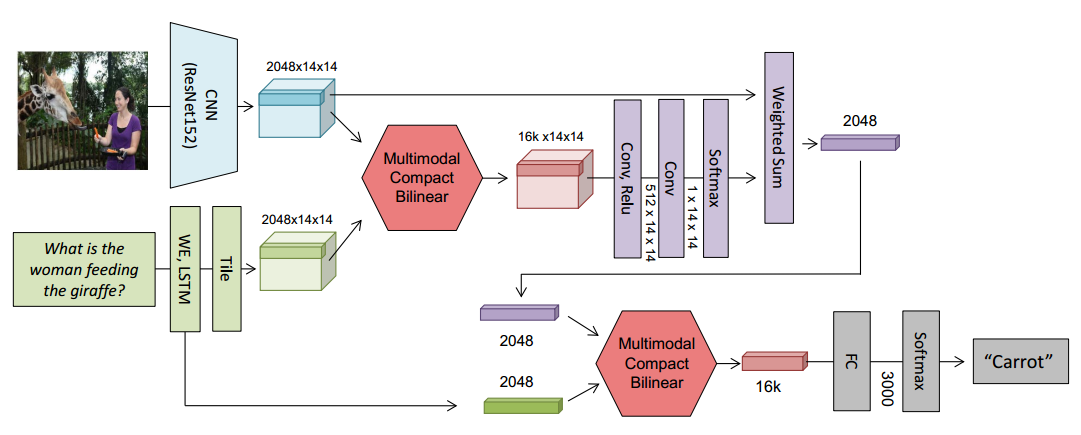
\includegraphics[width=1.0\linewidth]{mcbArch.PNG}
    	\caption{MCB architecture for the open-ended task of the VQA dataset.}
    	\label{mcbArch}
    \end{figure}
    \begin{figure}[ht]
    	\centering
            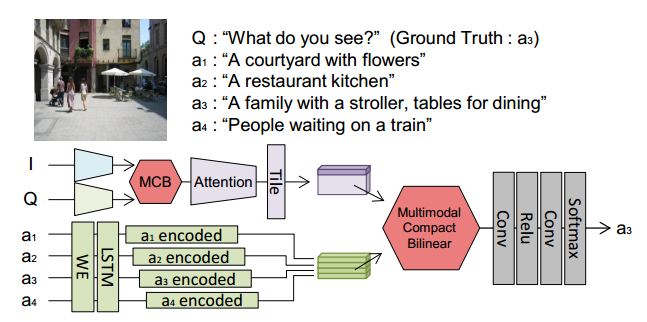
\includegraphics[width=0.75\linewidth]{mcbArch+ans.PNG}
        \caption{MCB architecture for the multiple-choice task of the VQA dataset.}
    	\label{mcbArch+ans}
    \end{figure}

\subsection{Experiments and Results}
The Adam solver with $e=0.0007, \beta_1=0.9, \beta_2=0.999$ is implemented and dropout after the LSTM layers and in fully connected layers is used. Also, early stopping is implemented if the validation score does not improve for 50,000 iterations. A value of $d = 16\,000$ for the higher dimension of the compact bilinear feature is adopted since it yielded the best accuracy results during training. The final results published correspond to an ensemble of 7 different methods, in which the authors experiment with different approaches such as augmenting the training data with images and QA pairs from the Visual Genome dataset or concatenating the learned word embeddings with pretrained GloVe vectors.

\section{DualNet: Domain-Invariant Network for VQA}\label{dualnetSec}
In this paper, Saito et al. \citep{corrSaito16} introduce DualNet, a model that attempts to fully exploit the discriminative information provided by the images and textual features, by separately performing addition and multiplication of input features to form a common embedding space. What makes DualNet remarkable is that unlike most of the other models, it does not use any attention mechanism. Furthermore, it is applicable to both real images and abstract scenes categories from the original VQA dataset.
\subsection{The Model}
The fusing of image features and text features by multiplication is performed as follows:
\begin{align*}
    I_{M_1} &= \text{tanh}(W_{M_1}I_1)\\
    I_{M_2} &= \text{tanh}(W_{M_2}I_2)\\
    I_{M_3} &= \text{tanh}(W_{M_3}I_3)\\
    Q_M &= \text{tanh}(W_{M_q}Q)\\
    F_M &= I_{M_1} \odot I_{M_2} \odot I_{M_3} \odot Q_M
\end{align*}
Where $Q$ is the question vector obtained from the last hidden layer of an LSTM over the embeddings of the question words, $I_k$ are the different image features considered for each image, and $\odot$ refers to element-wise multiplication.\\
Similarly, the fusing of features by summations is given by
\begin{align*}
    I_{S_1} &= \text{tanh}(W_{S_1}I_1)\\
    I_{S_2} &= \text{tanh}(W_{S_2}I_2)\\
    I_{S_3} &= \text{tanh}(W_{S_3}I_3)\\
    Q_S &= \text{tanh}(W_{S_q}Q)\\
    F_S &= I_{S_1} + I_{S_2} + I_{S_3} + Q_S
\end{align*}
The weights between multiplication and summation are not shared because it is expected that each operation extracts different kinds of information. Finally, the features are concatenated and pass through a final linear layer to generate the prediction of the model:
\begin{align*}
    F &= [F_M, F_S]\\
    Output &= W_{f_2} \text{tanh}(W_{f_1}F)
\end{align*}
The diagram for the DualNet architecture is depicted in figure \ref{dualnetArch}.

    \begin{figure}[ht]
    	\centering
            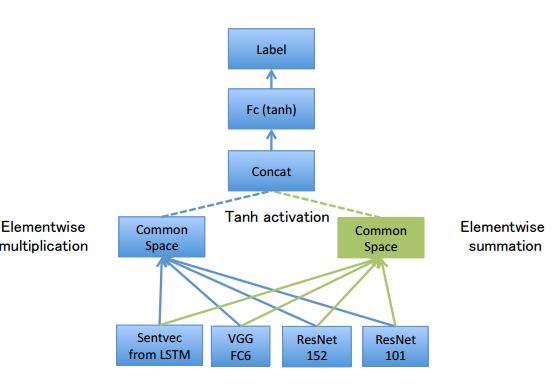
\includegraphics[width=0.75\linewidth]{dualnetArch.PNG}
        \caption{DualNet architecture.}
    	\label{dualnetArch}
    \end{figure}

\subsection{Experiments and Results}
The LSTM for the question consists of 2 layers with 512 units each. The 2,000 most frequent answers were used as labels and Rmsprop with learning rate 0.0004 and batch size 300 was used to optimize the model.\\
The three image features are taken as L2-normalized features from the first fully-connected layer of VGG19, and the uppermost fully-connected layers from ResNet-152 and ResNet-101.\\
The final results reported come from an ensemble of 19 DualNet units, where the common space for each unit is set differently in the range 500 to 3000.\\
The fact that the model achieves a good performance without any attention mechanism suggests that the image features from VGG and ResNet must contain a certain extent of spatial information that proves useful for the task at hand.

\section{Algorithms and Results Comparison}\label{resSec}
Table \ref{algos} shows a comparison of the different algorithms presented in previous sections. The following properties are worth noticing:
\begin{itemize}
    \item All algorithms use a variation of either VGGNet or ResNet (or both) to encode the input image features. This clearly shows the powerful nature of these two pre-trained CNNs when it comes to image processing.
    \item All algorithms excepting one use an RNN to encode the input question features. Most of them in the form of an LSTM and a couple in the form of a GRU. Similarly, to what happens with CNNs for images, RNNs have proven to be very effective to capture the information underlying a natural language text input. 
    \item Most algorithms implement some kind of attention mechanism, which helps focus on the parts of the question and image that are more relevant to the task at hand. Attention mechanisms have also been widely used for other tasks both in computer vision and NLP, yielding state-of-the-art results.
    \item Most algorithms use element-wise multiplication to bring together the image and question representations into a common feature space. This technique is probably the most straightforward one, but algorithms such as MCB which try to experiment with other kinds of multimodality mechanisms also perform extremely well.
\end{itemize}

Table \ref{results} shows a summary of the performances of the eight algorithms presented and compared in previous sections. As it is standard for the VQA dataset, there is an accuracy measure for each type of question (yes/no, number and other) in the test-dev open-answer and multiple-choice tasks, plus an overall accuracy measure for test-dev and test-std. Test-std results for the open-ended task can be compared to the first row in the table, which corresponds to the accuracy achieved by human annotators. Looking at this table it is easy to notice that
\begin{itemize}
    \item Multimodal Compact Bilinear Pooling (MCB) \citep{corrFukui16} has the best performance for all the results they published. This model was actually the winner of the 2016 VQA challenge, which proves that the method they introduce really excels in ways that others don't.
    \item Even though DualNet \citep{corrSaito16} is a very simple model which doesn't even incorporate an attention mechanism, it has a very good performance when compared to the rest of the algorithms. This is a clear example of how not only the model architecture but also the feature selection and extraction process is crucial to determine the performance of an algorithm.
    \item The category where all models struggle the most is numerical answers, which means that they are having trouble capturing enough information from the input image to accurately count instances of objects, although they might be doing a great job in differentiating presence or absence thereof.
\end{itemize}

    \begin{table}[ht]
    	\centering
    	\begin{tabular}{lllll}
    		\toprule
    		Model & Image & Question & Attention & Multimodality\\
    		\midrule
            LSTM Q+I \citep{iccvAntol15} & VGGNet (4096) & LSTM (1024) & --- & EWM \\
            HieCoAtt \citep{nipsLu16} & VGGNet (4096) & LSTM (1024) & Image + Question & EWM \\ 
            SAN \citep{corrYang15} & VGGNet (512) & CNN (1280) & Question & EWM \\
            MRN \citep{DBLP:corrKim16} & VGGNet (4096) & GRU (2400) & Implicit & EWM \\
            & ResNet (2048) & & & \\
            FDA \citep{corrIlievski16} & ResNet (2048) & LSTM (512) & Object Detection & EWM \\
            DMN \citep{corrXiong16} & VGGNet (512) & GRU (512) & Episodic Memory & EWM + \\
            & & & & Concatenation\\ 
            MCB \citep{corrFukui16} & ResNet (2048) & LSTM (2048) & MCB Pooling & MCB Pooling \\
            & & & & ($\Psi$ + FFT) \\ 
            DualNet \citep{corrSaito16} & ResNet152 & LSTM (1024) & --- & EWM + \\
            & ResNet101 & & & Summation\\
            & VGGNet19 & & & \\
    		\bottomrule
    	\end{tabular}
    	\caption{Algorithm comparison according to the representations used for image and question features, attention mechanism implemented and multimodality integration (EWM stands for Element-wise multiplication).}
        \label{algos}
    \end{table}

    \begin{table}[ht]
    	\centering
    	\begin{tabular}{lcccccccccc}
    		\toprule
    		& \multicolumn{5}{c}{Open-Ended} & \multicolumn{5}{c}{Multiple-Choice}\\ 
    		\cmidrule(lr){2-6} \cmidrule(lr){7-11}
    		& \multicolumn{4}{c}{test-dev} & test-std & \multicolumn{4}{c}{test-dev} & test-std\\ 
    		\cmidrule(lr){2-5} \cmidrule(lr){6-6} \cmidrule(lr){7-10} \cmidrule(lr){11-11}
    		Model & Y/N & Num & Other & All & All & Y/N & Num & Other & All & All\\
    		\midrule
    		Human & - & - & - & - & 83.3 & - & - & - & - & - \\
    		LSTM Q+I \citep{iccvAntol15} & 78.9 & 35.2 & 36.4 & 53.7 & 54.1 & 79.0 & 35.8 & 43.4 & 57.2 & - \\
    		HieCoAtt \citep{nipsLu16} & 79.7 & 38.7 & 51.7 & 61.8 & 62.1 & 79.7 & 40.0 & 59.8 & 65.8 & 66.1 \\
    		SAN \citep{corrYang15} & 79.3 & 36.6 & 46.1 & 58.7 & 58.9 & - & - & - & - & - \\
    		MRN \citep{DBLP:corrKim16} & 82.5 & 38.3 & 46.8 & 60.5 & 61.8 & - & - & - & - & 66.3 \\
    		FDA \citep{corrIlievski16} & 81.1 & 36.2 & 45.8 & 59.2 & 59.5 & 81.5 & 39.0 & 54.7 & 64.0 & 64.2 \\
    		DMN \citep{corrXiong16} & 80.5 & 36.8 & 48.3 & 60.3 & 60.4 & - & - & - & - & - \\
    		MCB \citep{corrFukui16} & \textbf{83.4} & \textbf{39.8} & \textbf{58.5} & \textbf{66.7} & \textbf{66.5} & - & - & - & \textbf{70.2} & \textbf{70.1} \\
    		DualNet \citep{corrSaito16} & 82.0 & 37.9 & 49.2 & 61.5 & 61.7 & \textbf{82.1} & \textbf{39.8} & \textbf{59.5} & 66.7 & 66.7 \\
    		\bottomrule
    	\end{tabular}
    	\caption{Results comparison of the different algorithms presented throughout the paper. Overall accuracy measures are presented for the test-dev and test-std partitions of the VQA original dataset for both open-ended and multiple-choice tasks. Additionally, accuracy per question type (Yes/No, Number and Other) is also provided for the test-dev partition. A value of "-" means that the result was not available in the original paper.}
        \label{results}
    \end{table}

\section{Making the V in VQA Matter: Elevating the Role of Image Understanding in Visual Question Answering}\label{newSec}
The biggest contribution of this paper \citep{cvprGoyal17} is the augmentation of the popular VQA dataset to make it more balanced by collecting complementary images such that every question is associated with not just a single image, but rather a pair of similar images that result in two different answers to the question. Some examples of this augmentation are depicted in figure \ref{balancedExample}.

    \begin{figure}[ht]
    	\centering
            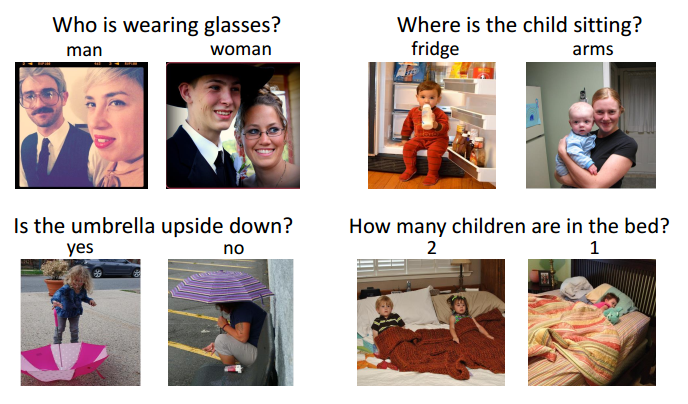
\includegraphics[width=0.75\linewidth]{balancedExample.PNG}
        \caption{Examples of the balanced VQA dataset.}
    	\label{balancedExample}
    \end{figure}

When testing a number of VQA models on this balanced dataset, all of them perform significantly worse, suggesting that these models are learning to exploit language priors instead of actually interpreting the nuances of the image.\\
To create the balanced dataset, given an (image, question, answer) tuple $(I,Q,A)$ from the original VQA dataset, a human subject is asked to identify an image $I'$ that is similar to $I$ but results in the answer to the question $Q$ to become $A' \neq A$. Under these conditions, since the same question $Q$ has two different answers for two different images, the only way for a model to know the right answer is by looking at the image.\\
The balanced VQA dataset is also particularly difficult because $I'$ is close to the original image $I$ in the semantic space of VGGNet features. Thus, VQA models must capture subtle differences between the two images to predict both answers correctly.
\subsection{The Dataset}
Using Amazon Mechanical Turk (AMT), human subjects are shown 24 nearest-neighbor images of $I$, the question $Q$ and the answer $A$. They are asked to pick an image $I'$ for which $Q$ makes sense and the answer is not $A$. The 24 nearest-neighbors are computed by representing each image with the activations of the penultimate layer of VGGNet and then $L_2$-distances are used to calculate vicinity. Finally, $I'$ and $Q$ are shown to 10 new AMT subjects to collect 10 ground truth answer. The most common answer among the 10 is the new answer $A'$.\\
If the question does not make sense for any of the 24 images, or the answer is still $A$ for all applicable neighboring images, the subjects were allowed to pick the option "not possible". Therefore, the resulting dataset is not perfectly balanced, but it is significantly more balanced than the original VQA dataset. In particular, the entropy of the answer distributions averaged across various question types increases by 56\% after balancing, which confirms the heavier tails in the answer distribution. Figure \ref{balancedAns} shows the answer distribution for the balanced dataset (compare to figure \ref{ansdist}). 

    \begin{figure}[ht]
    	\centering
            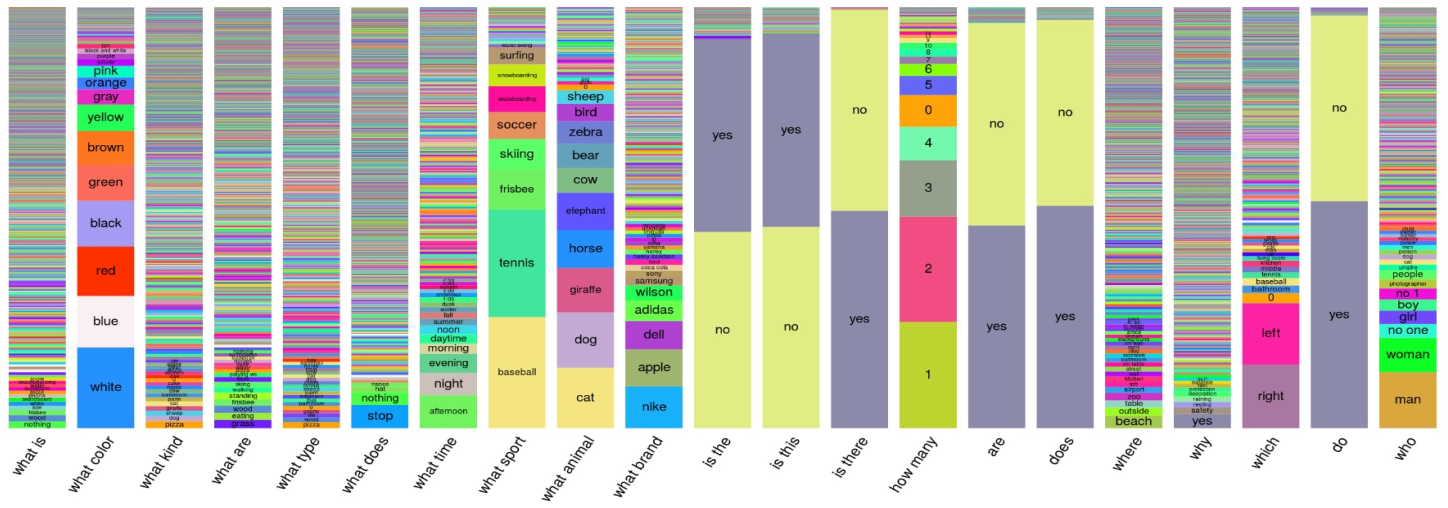
\includegraphics[width=1.0\linewidth]{balancedAns.PNG}
        \caption{Distribution over the answers of the balanced VQA dataset for different kinds of questions.}
    	\label{balancedAns}
    \end{figure}

\subsection{Benchmarking Existing VQA Models}
Taking as reference a prior model (always predicts the most common answer in the training set) and a language-only model (does not use any visual information), table \ref{vqa2} shows the degradation in performance for the three models proposed in \citep{iccvAntol15}, \citep{nipsLu16} and \citep{corrFukui16}.

    \begin{table}[ht]
    	\centering
    	\begin{tabular}{rcccc}
    		\toprule
    		Model & UU & UB &  $\text{B}_{\text{half}}$B & BB\\
    		\midrule
            Prior  & 27.38 & 24.04 & 24.04 & 24.04\\
            Language-only & 48.21 & 41.40 & 41.47 & 43.01\\
            LSTM Q+I \citep{iccvAntol15} & 54.40 & 47.56 & 49.23 & 51.62\\
            HieCoAtt \citep{nipsLu16} & 57.09 & 50.31 & 51.88 & 54.57\\
            MCB \citep{corrFukui16} & 60.36 & 54.22 & 56.08 & 59.14\\
    		\bottomrule
    	\end{tabular}
    	\caption{Performance of VQA models when trained/tested on unbalanced/balanced VQA datasets. UB stands for training on Unbalanced train and testing on Balanced val datasets. UU, $\text{B}_{\text{half}}$B and BB are defined analogously.}
        \label{vqa2}
    \end{table}

It is worth noticing that the accuracy of all models improves by 2-3\% when they are trained on the complete balanced dataset B compared to when they are trained using only half of it ($\text{B}_{\text{half}}$). This increase in accuracy suggests that the models are data starved and would benefit from even larger VQA datasets.
\subsection{Counter-examples Model}
Built on top of a regular VQA model, the focus of the counter-examples model is to make the VQA model more trustworthy by providing an explanation of the decision made, i.e. an example image that is similar to the input image, but the model believes has a different answer to the input question. For example, if the question is "What color is the fire-hydrant?", the VQA model could respond "red" and additionally (through the counter-examples model) show an example image containing a fire-hydrant that is not red.\\
This additional module, called the explaining head, must learn to explain an answer $A$ via a counter-example image. It is modeled as a 2-channel network which linearly transforms the joint $QI_k$ embedding and the answer to be explained $A$ into a common embedding space. The joint $QI_k$ embedding is calculated for all $I$ in the set $I_{NN}$, conformed by the $K$ nearest neighbor images of the original input image $I$. An inner product of the two embeddings ($QI_k$ and $A$) result in a scalar number for each image in $I_{NN}$. These $K$ values are passed through a fully connected layer to generate $K$ scores $S(I_k)$ that are used to sort the candidate images as being most to least likely of being good counter-examples or negative explanations.\\
Figure \ref{balancedCounter} shows an example of the results generated by the explaining head module.

    \begin{figure}[ht]
    	\centering
            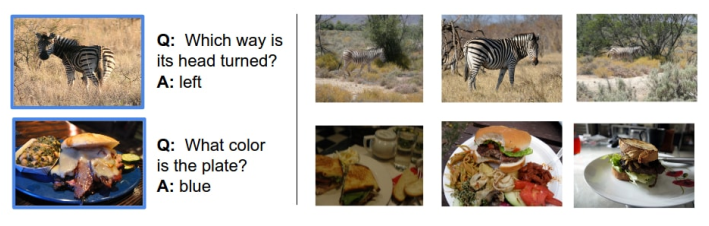
\includegraphics[width=1.0\linewidth]{balancedCounter.PNG}
        \caption{Instances of the counter-examples generated by the explaining head of the balanced VQA model.}
    	\label{balancedCounter}
    \end{figure}

\section{Future Work}\label{futureSec}
Possible lines of work that arise from studying the results in section \ref{resSec} and the new VQA dataset proposed in section \ref{newSec} are the following:
    \begin{itemize}
        \item Explore algorithms that focus on a counting mechanism, since the accuracy for questions with a numerical answer is the worst throughout all the algorithms presented thus far.
        \item Building on top of the MCB model, which yielded the best results among the algorithms presented on this paper. For instance, trying to apply MCB instead of element-wise multiplication in some of the other algorithms to see if their accuracy can be improved.
        \item Another alternative for the element-wise multiplication approach could be to use Kernel methods. Before computing the element-wise product, a kernel function could be applied to each feature (which would project the common space to a higher dimension, similarly to what is achieved with MCB) therefore obtaining a potentially richer representation of the multimodal problem.
        \item Creating an ensemble method, which integrates the different approaches presented in this paper (and others), could potentially result in a more robust classifier that benefits from the different natures of all the underlying algorithms.
        \item Modifying the existing algorithms to take into consideration the original bias of the VQA dataset, in order to improve their performance in the new version. More specifically, the modified algorithms should pay special attention to the input image, since it becomes the sole differentiator when any given question can have multiple correct answers.
    \end{itemize}

\section{Conclusions}\label{conclusions}
In this paper we presented a comprehensive compilation of basic algorithms released in recent years for the Visual Question Answering problem.\\
We covered the standard approach throughout the literature, which maps the vector representations of questions and images to a common feature space, and analyzed its most popular implementations. We also explained the improvements introduced by several authors that build on top of this concept, such as attention mechanisms, episodic memory and compact bilinear pooling.\\
Additionally, we explored the most common dataset used in recent years to develop VQA algorithms and assess their accuracy, with an emphasis on how it was designed and constructed, the type of questions and answers it includes and recent efforts that have been made to improve it by reducing its imbalance and bias.\\
Finally, we presented a number of promising directions for future research. In particular, we suggest the inclusion of other machine learning techniques such as kernels and ensemble methods, which have previously proven its effectiveness in similar applications. A continued exploration of NLP and CV processing tools will also be of paramount importance, since they lie at the core of the VQA task.

% \nocite{*}
\bibliography{main} % path to your bib file (without .bib extension!)
% \bibliographystyle{plainnat} % bib style (IEEE, APA, etc.)
\bibliographystyle{ieeetr} % bib style (IEEE, APA, etc.)
%\bibliographystyle{ksfh_nat} % bib style (IEEE, APA, etc.)

\end{document}
